% Here we have your executive summary.
This thesis describes a new method for measuring strain dependent surface stress in soft solids, as well as the corresponding measurements for two silicone polymer gels. Over the past several years, recent attempts to measure surface stress in gels have returned a cornucopia of conflicting results, differing significantly in similar materials. Recently, Xu, Jensen et al. suggested that this discrepancy is an artifact of the strain state of the gels, and made the first measurement of strain-dependent surface stress, $\Upsilon(\epsilon)$, in solids \cite{xu2017direct}. In this paper, the authors reported that the surface stress changed dramatically under applied strain. At 18\% strain, the surface stress more than doubled. This dramatic change in surface stress was a surprising result. 
\begin{figure}[h!]
	\centering
%	\textbf{Should I give it a title?}\par\medskip
	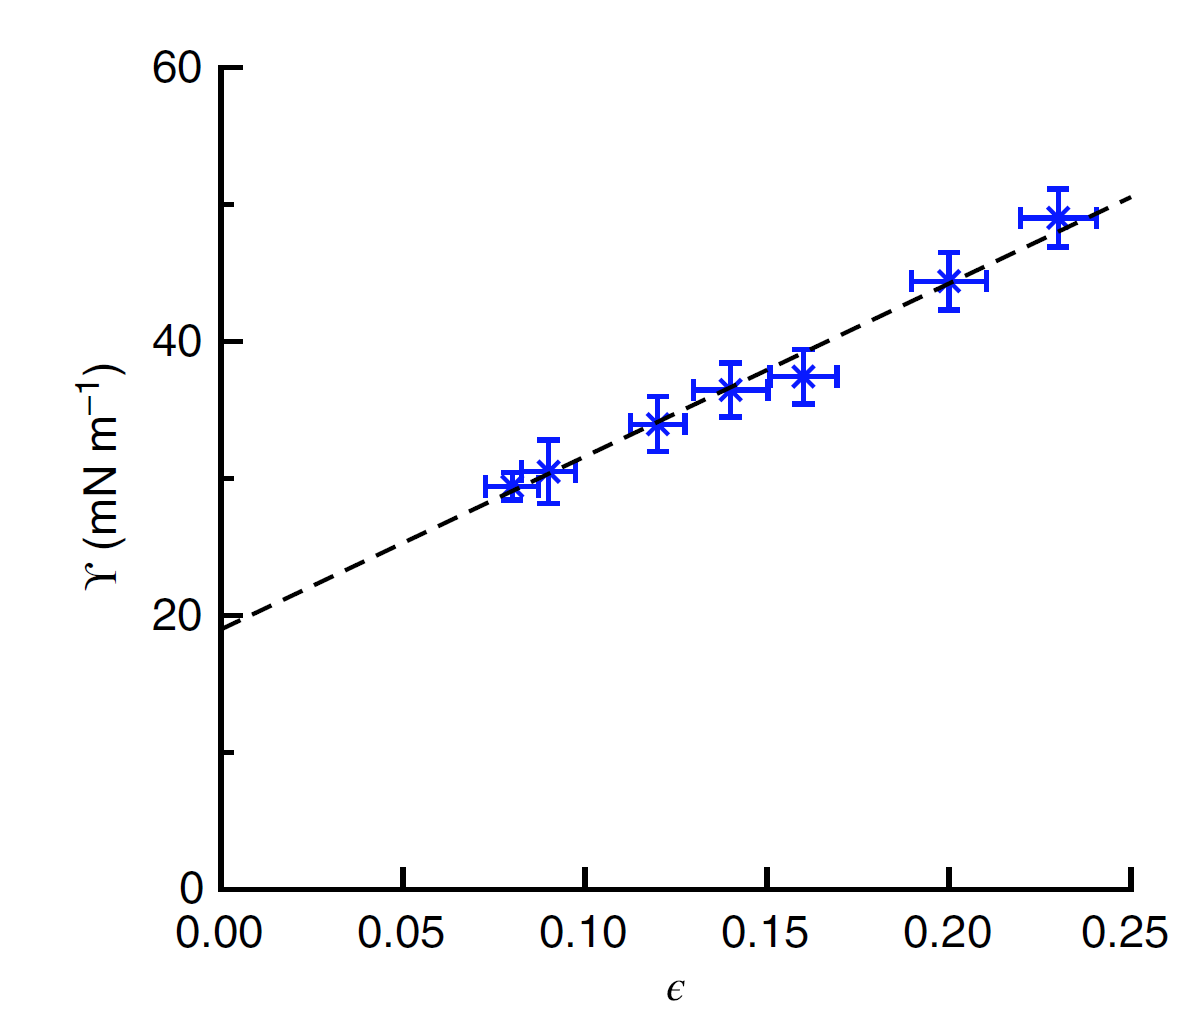
\includegraphics[width=0.69\linewidth]{Chapters/Figures/2017natcomfig}
	\caption[Surface Stress vs. Strain in Silicone]{This is first direct measurement of strain dependent surface stress in solids \cite{xu2017direct}. Using a compliant silicone gel, surface stress, $\Upsilon$, was found to grow linearly as a function of strain, $ \epsilon $.}
	\label{fig:2017natcomfig}
\end{figure}

Over the past year, we have helped develop a new method for measuring $\Upsilon(\epsilon)$ and $ W(\epsilon) $ in soft solids. By measuring the spontaneous indentation depth of rigid spheres over a range of sizes, we can calculate $ \Upsilon $ and $ W $ using theory derived from our understanding of soft adhesion. Our adhesion-based technique can be applied to a wide variety of stretchable materials. Additionally, we have built our own equibiaxial stretching apparatus, improving upon the earlier published design \cite{xu2017direct} to produce nearly twice the strain in identical materials. Using this technique, we have measured the adhesion energy and surface stress in two types of silicone, as well as preliminary $ \Upsilon(\epsilon) $ measurements as we work towards recreating the surprising 2017 measurement.

Our $ \Upsilon $ and $ W $ measurements for PDMS on glass (zero applied strain) are encouraging. Measurements of spontaneous indentation depth, d vs. the radius of return solid fits with minimal noise. Additionally, the calculated values values for $ \Upsilon $ and $ W $ agree with previous measurements. 

\begin{figure}[h!]
	\centering
	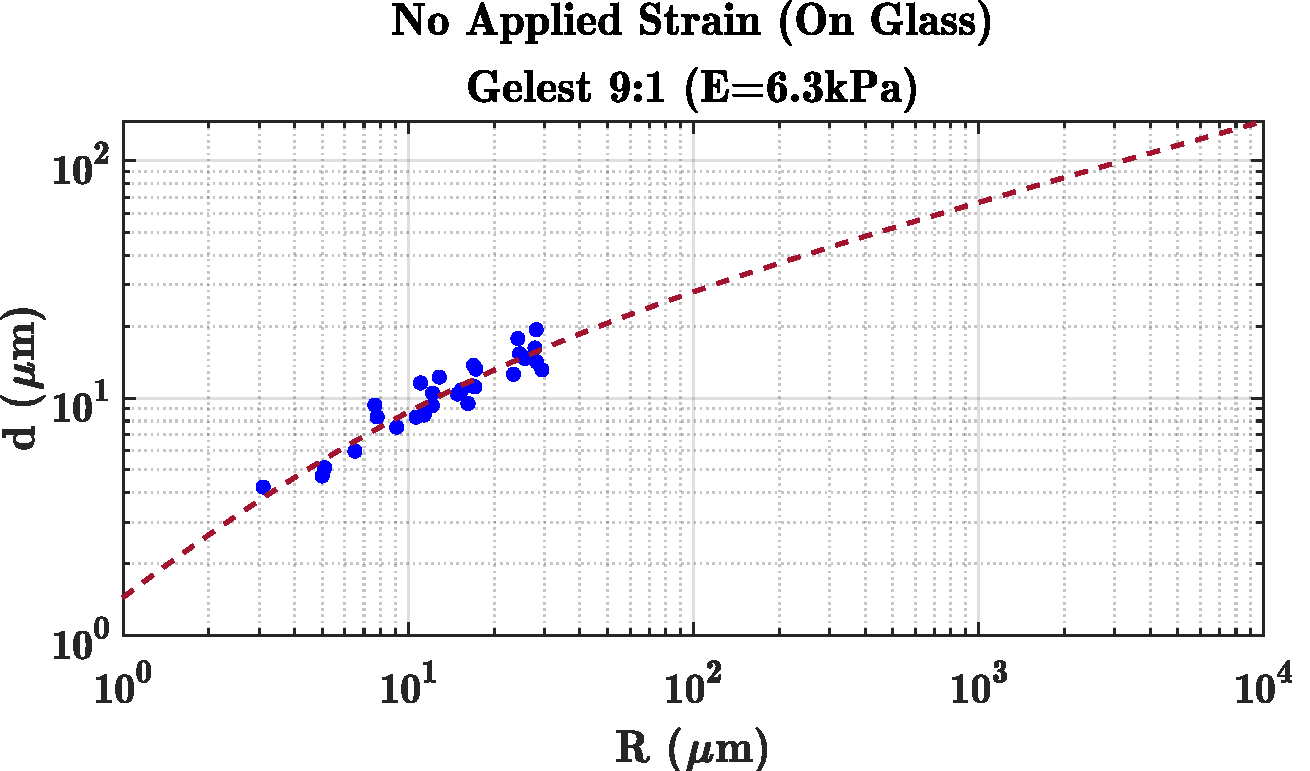
\includegraphics[width=\linewidth]{Chapters/Figures/w_ups_fit_G9-1}
	\caption[Gelest W-$\Upsilon$ Fit]{We plot the spontaneous indentation depth, d, vs. radius, R, for many silica beads sinking into a soft silicone substrate. By considering the elastocapillary adhesive forces acting on the sphere, we fit an equation (Equation \ref{THEeqn}) using to the d vs. R plot for a Gelest silicone sample. The best fit line returns parameters of $ W=53 $  and $ \Upsilon=32 $ mNm$^{-1}$.}
	\label{fig:wupsfitg9-1}
\end{figure}

Currently, the depth vs. radii measurements for PDMS on a stretchable substrate contain a significantly greater amount of noise than for the same substrate adhered to glass. Until the noise level is reduced, we cannot fit our data to extract $ \Upsilon $ and $ W $ values. However, our preliminary results suggest that the surface stress in gels does significantly change under strain. The figure demonstrates visually this $ \Delta\Upsilon $ for a single silica sphere sitting into a silicone substrate. As the underlying gel is stretched, the surface tension increases, reducing the depth into which the sphere sits. 
\begin{figure}[h!]
	\centering
	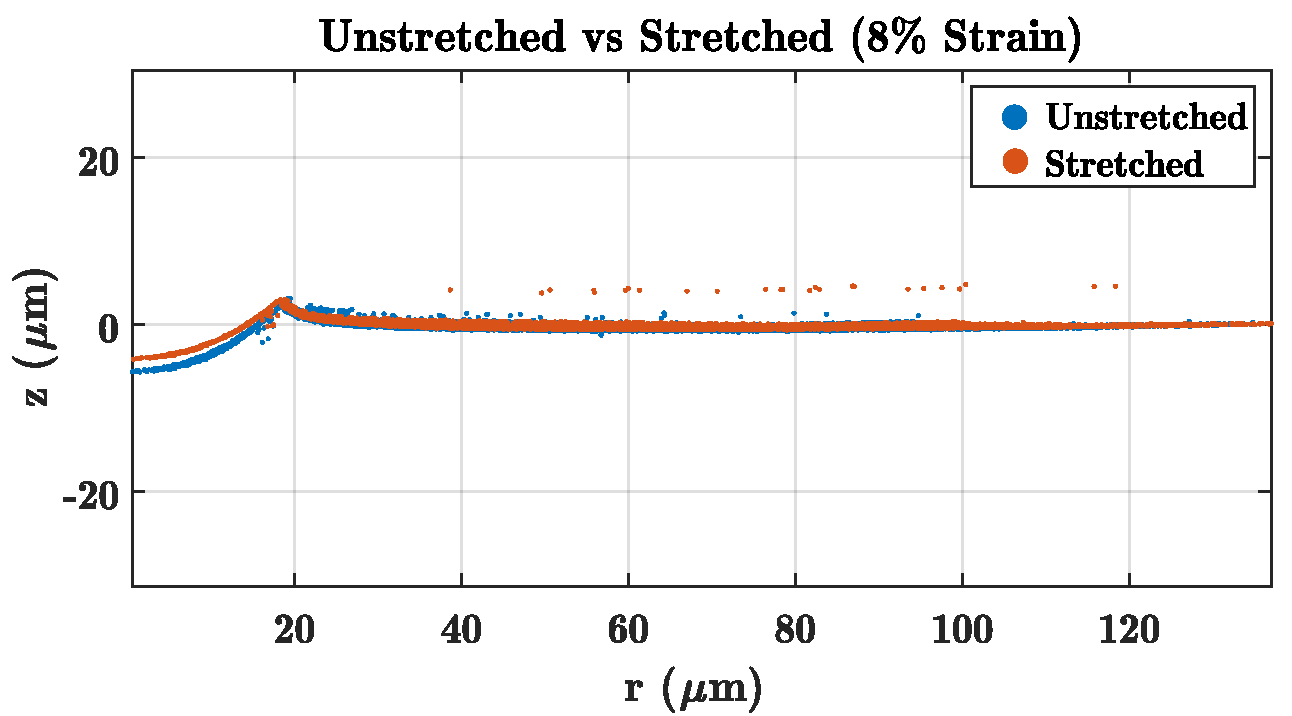
\includegraphics[width=\linewidth]{Chapters/Figures/sc1_unstretched_v_8ml_cropped}
	\caption[Side Collapse Comparison]{The side profile of the same silica sphere sitting in a silicone substrate before and after stretch. When a strain is applied, the sphere's indentation into the substrate is shallower. Substrate is Gelest PDMS with stiffness $\text{E}=6.3$ kPa.}	
	\label{fig:sc1unstretchedv8ml}
\end{figure}




\todo[inline, color=orange]{Re-analyze this data to make sure scaling is correct!.}

